\tikzstyle{circular} = [draw, circle, minimum size=.3cm, node distance=1.75cm]
\tikzstyle{arrow}=[->, thick, shorten <= 2pt, shorten >= 2pt]

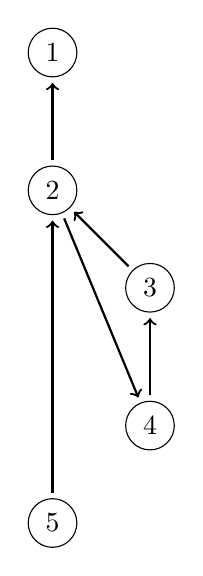
\begin{tikzpicture}[level/.style={thick}]
  \node[circular](one)   {1};
  \node[circular, below of = one](two)   {2};
  \node[circular, below right of = two](three) {3};
  \node[circular, below of = three](four)  {4};
  \node[circular, below left of = four](five)  {5};

  \draw[arrow] (two) to (one);
  \draw[arrow] (three) to (two);
  \draw[arrow] (four) to (three);
  \draw[arrow] (two) to (four);
  \draw[arrow] (five) to (two);

\end{tikzpicture}
